\documentclass[letterpaper,11pt]{article}

\usepackage{listings}
\usepackage{color}

\definecolor{dkgreen}{rgb}{0,0.6,0}
\definecolor{gray}{rgb}{0.5,0.5,0.5}
\definecolor{mauve}{rgb}{0.58,0,0.82}

\lstset{frame=tb,
  language=Python,
  aboveskip=3mm,
  belowskip=3mm,
  showstringspaces=false,
  columns=flexible,
  basicstyle={\small\ttfamily},
  numbers=none,
  numberstyle=\tiny\color{gray},
  keywordstyle=\color{blue},
  commentstyle=\color{dkgreen},
  stringstyle=\color{mauve},
  breaklines=true,
  breakatwhitespace=true,
  tabsize=3
}

\usepackage{setspace}
\usepackage{graphicx}
\usepackage{bm}    %for textbf
\usepackage{amsmath}
\usepackage{amsfonts}   %for mathbb
\allowdisplaybreaks[4]  %from {amsmath}
\newcommand{\independent}{\rotatebox[origin=c]{90}{$\models$}}  %from {graphicx}
\usepackage{geometry}
\geometry{letterpaper, scale=0.8}  %from {geometry}
\author{Yuan Yin}
\title{MATH 623 Homework 2}
\begin{document}\large
\maketitle
\begin{spacing}{1.2}  %from {setspace}
\section*{Problem 3}
\subsection*{5.}
The main code:
\begin{lstlisting}
T = 1; K = 1; r = 0.02; delta = 0.3; N = 1000; M = 10^5;
s_bar = K * exp(3 * delta * T^(0.5) / K^(0.5) + abs(r - delta^2 * 0.5 / K) * T);
dt = T / M; ds = s_bar / N; p = zeros(N+1, M+1);
for i = 1 : (N + 1)
    p(i, M + 1) = max(ds * (i - 1) - K, 0);
end
for i = 1 : (M + 1)
    p(N + 1, i) = s_bar - exp(-r * (T - dt * (i - 1))) * K;
    p(1, i) = 0;
end
for i = (M + 1) : -1 : 2
    for j = 2 : N
        alpha1 = 1 - delta^2 * (j - 1) * dt / ds;
        alpha2 = delta^2 * (j - 1) * dt * 0.5 / ds + r * (j - 1) * dt * 0.5;
        alpha3 = delta^2 * (j - 1) * dt * 0.5 / ds - r * (j - 1) * dt * 0.5;
        p(j, i - 1) = alpha1 * p(j, i) + alpha2 * p(j + 1, i) + alpha3 * p(j - 1, i);
    end
end
s = 0 : ds : s_bar;
plot(s, p(:,1))
\end{lstlisting}
the plot of $P(s,0)$ is as below:

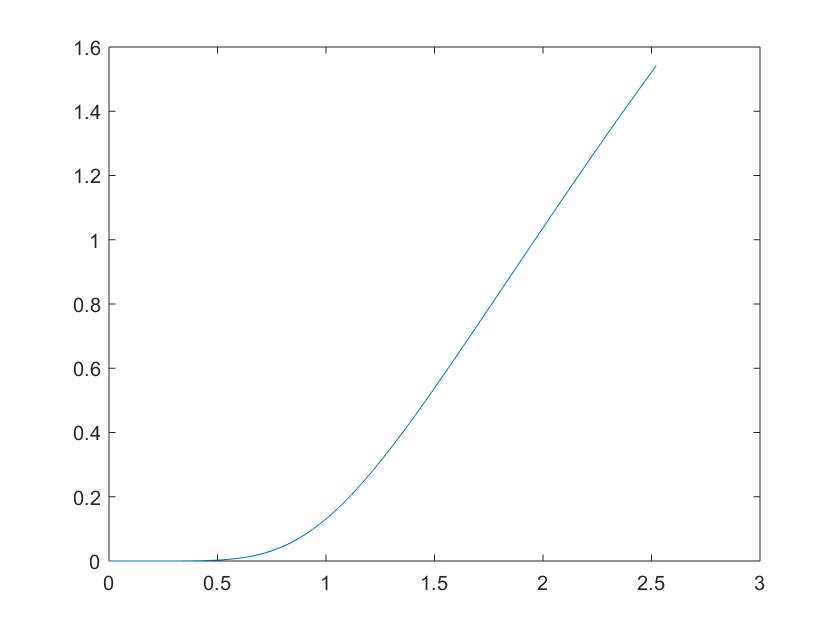
\includegraphics[width=4.95in,height=4.05in]{p_s_0.jpg}
\end{spacing}
\end{document}